\section{System Design}
\label{sec:system-design}

In this section, we dive into each component of \sysname{}; we focus on
degradation and adaptation, rather than being verbose on every component.

Applications in \sysname{} are composed by connecting a set of operators to form
a dataflow processing graph. Our system provides basic set of APIs such as
\texttt{map}, \texttt{filter}, \texttt{window} (\autoref{tab:operators}). The
normal operators are similar to existing stream processing systems; our
contribution is the set of APIs to allow the specification of degradation
operations for bandwidth-accuracy trade-off.

\begin{table*}
  \centering
  \begin{tabular}{ c r l }
    \toprule
    \multirow{7}{*}{Normal Operators}
    & \textit{map}(f: I $\Rightarrow$ O) & Stream<I> $\Rightarrow$ Stream<O> \\
    & \textit{filter}(f: I $\Rightarrow$ bool) & Stream<I> $\Rightarrow$
                                                 Stream<I> \\
    & \textit{skip}(i: Integer) & Stream<I> $\Rightarrow$ Stream<I> \\
    & \textit{sliding\_window}(count: Integer, f: Vec<I> $\Rightarrow$ O) & Stream<I> $\Rightarrow$
                                                                            Stream<O> \\
    & \textit{tumbling\_window}(count: Integer, f: Vec<I> $\Rightarrow$ O) & Stream<I> $\Rightarrow$
                                                                             Stream<O> \\
    & \textit{timed\_window}(time: Duration, f: Vec<I> $\Rightarrow$ O) & Stream<I> $\Rightarrow$
                                                                          Stream<O> \\
    & ... & ... \\
    \midrule
    \multirow{4}{*}{Degradation Operators}
    & \textit{maybe}(knobs: Vec<T>, f: (T, I) $\Rightarrow$ I) & Stream<I> $\Rightarrow$
                                                                 Stream<I> \\
    & \textit{maybe\_skip}(knobs: Vec<T>) & Stream<I> $\Rightarrow$ Stream<I> \\
    & \textit{maybe\_downsample}(knobs: Vec<(Integer, Interger)>) & Stream<Image> $\Rightarrow$ Stream<Image> \\
    & ... & ... \\
    \bottomrule
  \end{tabular}
  \caption{A comparison between normal stream processing operators and our
    degradation operators. Vec<T> represents a list of elements of type
    T. Option<T> indicates an element of type T can be absent. Notice the type
    constrain on the \texttt{maybe} function while \texttt{maybe\_map} relaxes
    it.}
  \label{tab:operators}
\end{table*}

\subsection{Degradation Operators}
\label{sec:prog-abs}

We first consider a strawman solution: manual policies for
degradation. JetStream~\cite{rabkin2014aggregation} offers an example: ``if
bandwidth is insufficient, switch to sending images at 75\% fidelity, then 50\%
if there still isn't enough bandwidth. Beyond that point, reduce the frame rate,
but keep the images at 50\% fidelity.'' We identify the following issues with
this approach.

\para{Lack of precision:} These policies are often developer heuristics and
rarely backed up by measurements. First, there is no direct association of the
application accuracy with the 75\% fidelity configuration. Besides, their impact
on the data size is also not trivial.  While it seems intuitive that the level
of degradation will affect the data size, the precise impact is not always
straightforward. For example, one might think that reducing the frame rate by
50\% will half the data rate. When video encoding is employed, the inter-frame
difference will increased (P-frame size) when the frame rate is reduced. This
leads to a larger data size for each frame. \autoref{fig:h264} illustrates this
complex relationship with an example of H.264 encoding under four different
frame rates.

\para{Not scalable:} The strawman solution quickly leads to too many policies
when multiple degradation operations are involved or a fine-grained control is
desired. This manual process becomes tedious and error-prone. When too few rules
are provided, the application may oscillate between two rules: one that's too
aggressive (always faces insufficient bandwidth) and one that's too
conservative.

\begin{figure}
  \centering
  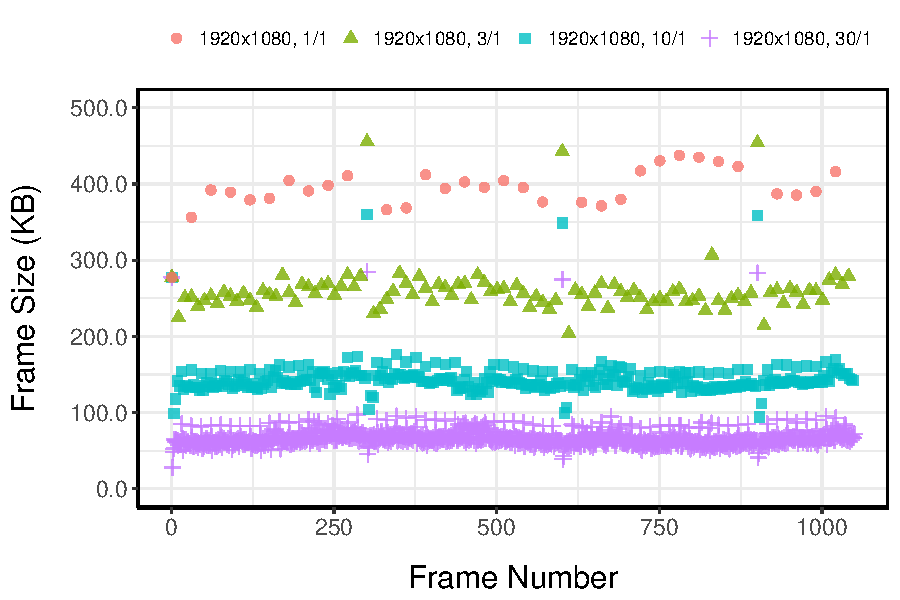
\includegraphics[width=\columnwidth]{figures/h264.pdf}
  \caption{H.264 requires more information per frame when the frame rate is
    reduced.}
  \label{fig:h264}
\end{figure}

\vspace{0.5em}

When using the above strawman solution, developers are forced to manually study
and measure the impact of individual degradation policy, prohibiting its wide
adoption in practice.

On the other extreme of the design spectrum, a completely developer-free
solution is not practical. While static analysis has been shown to optimize
application execution adaptively in a certain context~\cite{chun2011clonecloud},
they do not work well in our dataflow programming model. Static analysis is
prone to false positives: exploring wrong or unnecessary parameters. For
example, when the application is configured to generates statistics with a
\texttt{timed\_window} operation, static analysis may falsely detect the
duration parameter and alter the behavior of the application in an unexpected
way. Also, as we will illustrate in~\autoref{sec:profiling}, with each
introduced parameter, the profiling time increases drastically as all parameters
pose a combinatorial space.

Our system take a middle ground between these two extremes: developers use a
novel \texttt{maybe} API to annotate degradation operations without being exact
on the values. Think of these APIs as hints from developers: this operation,
when in use, will likely reduce the data size and affect the data fidelity;
however the exact impact is not clear.

The basic form of \texttt{maybe} operator takes two arguments: a knob and a
degradation function (see \autoref{tab:operators}). The knob indicates different
degradation levels; the function performs the actual degradation operation with
a configurable level. We restrict the type signature of the function that this
API can accept: $f(T, I) \Rightarrow I$. That is, the degradation function
should not alter the type of the stream. While this might seem a strong
restriction, when combined with \texttt{map} operator, the system is still
expressive enough. We describe our implementation and usage
in~\autoref{sec:implementation}.

\begin{sloppypar}
  Based on the \texttt{maybe} primitive, one can implement wrappers for common
  degradation operations. For example, \texttt{maybe\_skip} will optionally
  subsample a stream; and \texttt{maybe\_downsample} can adjust the image
  resolution to a configured target. With this API, the example mentioned
  earlier can now be implemented as follows:
\end{sloppypar}

\begin{lstlisting}
   let app = Camera::new((1920, 1080, 30))
      .maybe_downsample(vec![(1600, 900), (1280, 720)])
      .maybe_skip(vec![2, 5])
      .map(|frame| frame.show())
      .compose();
\end{lstlisting}

This snippet first instantiate a \texttt{Camera} source, which is a
\texttt{Stream<Image>} with 1920x1080 resolution and 30 FPS. Two degradation
operations are chained after the source: one that downsample the resolution to
either 1600x900 or 1280x720; the other skip the frame with a parameter of 2 or
5, resulting in 30/(2+1)=10 FPS or 30/(5+1)= 6 FPS. After the degradation,
images are shown on the display. In practice, further processing operators can
be chained.

While the API itself has simplified the specification of degradation, the exact
amount has to be known for precise rate adjustment at runtime. We then turn to
the second stage of our system that performs automatic profiling.

%%% Local Variables:
%%% mode: latex
%%% TeX-master: "sigcomm2017"
%%% End:
